% !TeX spellcheck = nl_NL
\documentclass[a4paper,kul]{kulakarticle} %options: kul or kulak (default)

\usepackage[utf8]{inputenc}
\usepackage[dutch]{babel}

\date{Academiejaar 2021 -- 2022}
\address{
	Industriële Ingenieurswetenschappen \\
	BioTechnologie \\
	Inge Holsbeeks \& Hans Rediers}
\title{Samenvatting}
\author{Robbe Decapmaker}
\usepackage{hyperref}
\usepackage{graphicx}
\usepackage{amsmath, amssymb, amsthm}
\usepackage{siunitx}
\usepackage{flafter} 
\usepackage{pdfpages}



\begin{document}

\maketitle

\section*{Inleiding}

De samenvatting van BioTechnologie. \href{https://github.com/debber1/BioTech}{De source code is te vinden op Github.}\\
%DEZE ZIN IS ENKEL RELEVANT TIJDENS DE ONTWIKKELING VAN DIT DOCUMENT
\textbf{Dit document is een `work in progress', dit wil zeggen dat er (ongeveer) een wekelijkse update zal zijn. De meest recente versie zal altijd op Github staan!}
\tableofcontents
\newpage
\section{Koolhydraten}
Koolhydraten zijn essentieel voor biologisch leven. Grosso modo kunnen we 3 verschillende types onderscheiden: monosachariden, disachariden en polysachariden. Voor dat we deze types degelijk kunnen bespreken moet er eerst enkele afspraken vast gelegd worden rond naamgeving een voorstelling. We moeten ook nog enkele belangrijke opmerken maken rond de chemische fenomenen die zich voor doen bij koolhydraten. 
\subsection{Naamgeving}
Koolhydraten bestaan voornamelijk uit C, O en H atomen. Afhankelijk van de onderling gevormde bindingen kunnen we een onderscheid maken tussen twee soorten koolhydraten; de aldosen en ketonen. Het verschil tussen beiden wordt duidelijk gemaakt in figuur \ref{fig:aldehyde-keton}. Als een koolhydraat in bezit is van een aldehyde groep, noemen we hem een aldose. Als hij in bezit is van een keton groep, noemen we hem een ketose.
\begin{figure}[htbp]
	\centering
	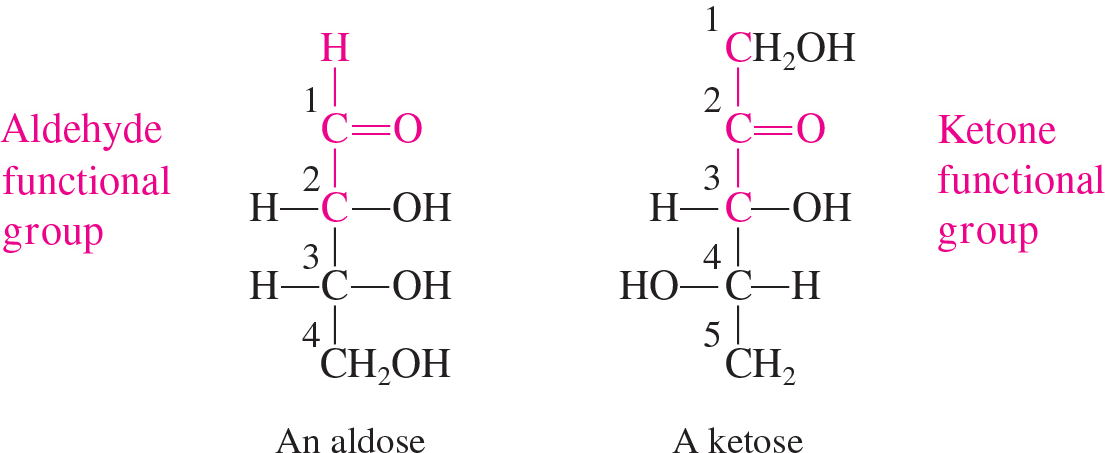
\includegraphics[width=0.7\linewidth]{Aldehyde-Keton}
	\caption[Aldehyden en ketonen]{Aldehyden en ketonen}
	\label{fig:aldehyde-keton}
\end{figure}\\
Naast de aanwezigheid van functionele groepen, maken we ook een onderscheid op basis van het aantal aanwezige koolstof atomen. De nummering en naamgeving van deze moleculen worden overgenomen uit de chemie zoals te zien is op figuur \ref{fig:examples-name}.
\begin{figure}[htbp]
	\centering
	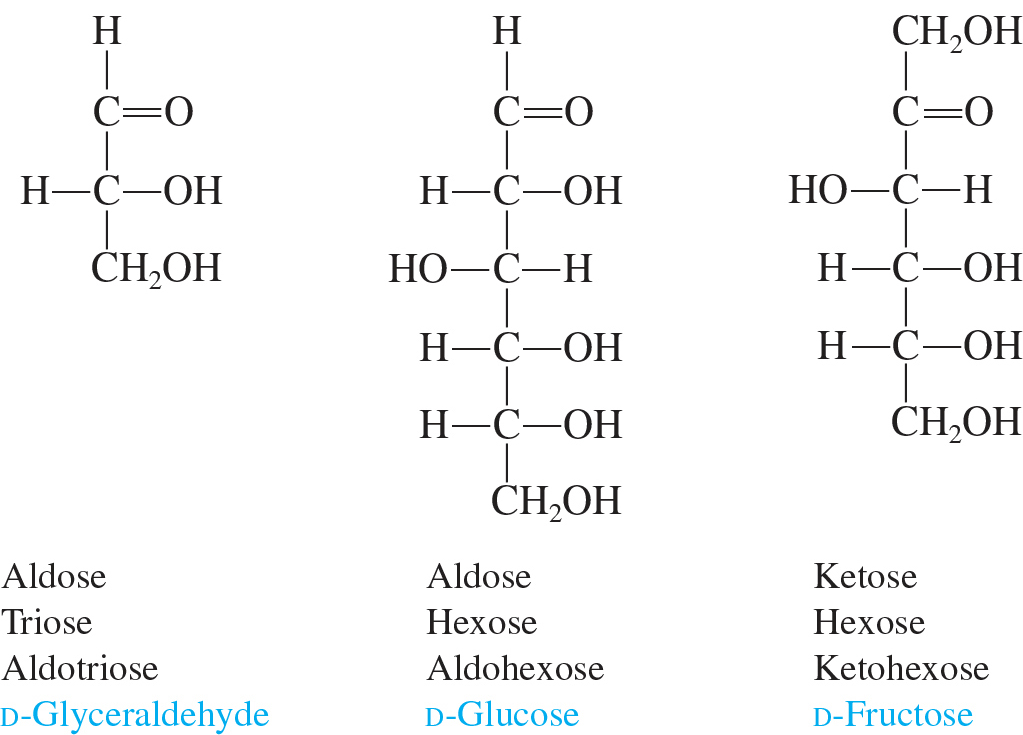
\includegraphics[width=0.6\linewidth]{examples-name}
	\caption[Naamgeving]{Voorbeelden van naamgeving}
	\label{fig:examples-name}
\end{figure}\\
Er zijn ook enkele koolhydraten die een triviale naam krijgen, zoals sacharose of fructose.

\subsection{Voorstellingen}
Er bestaan twee manieren om een koolhydraat voor te stellen, de Fischer- en Haworthprojectie. Voor D-glucose zien we op figuur \ref{fig:fishervshaworth} beide voorstellingen.
\begin{figure}[h]
	\centering
	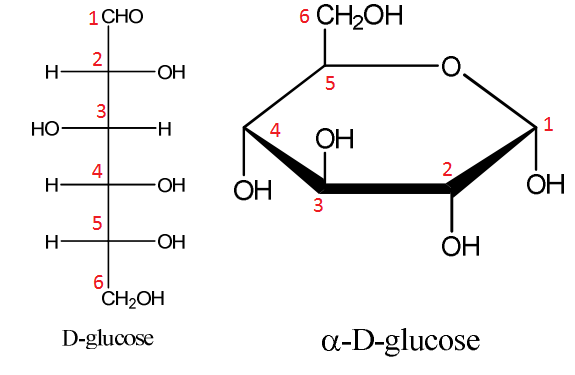
\includegraphics[width=0.6\linewidth]{FisherVSHaworth}
	\caption[Fischer- en Haworthprojectie]{Fischerprojectie (links) en Haworthprojectie (rechts)}
	\label{fig:fishervshaworth}
\end{figure}

\subsection{Stereochemie}
Als de structuur van een koolhydraat koolstof atomen bevat die gebonden zijn met vier verschillende groepen, zeggen we dat de structuur een chiraal centrum heeft. Dit fenomeen kan tot opmerkelijke resultaten leiden, zo is het mogelijk da bepaalde functionele groepen niet altijd op dezelfde manier georiënteerd zijn.  
\subsubsection{Enantiomeren}
We spreken van enantiomeren als een we te maken hebben met een molecule die volledig gespiegeld kan worden. Een voorbeeld is te zien op figuur \ref{fig:enantiomeren}. Deze spiegeling heeft enkele gevolgen, zowel op biologisch als op fysisch vlak. Zo kunnen verschillende enantiomeren anders reageren op gepolariseerd licht. Vanuit een biologisch standpunt vormt er een probleem als de enantiomeren niet op dezelfde manier samenwerken met enzymen (zie figuur \ref{fig:enantiomeerenzym}). Als beide enantiomeren (normaal en gespiegeld of L en D in een biologische context) aanwezig zijn in een mengsel, dan nomen we dit een racemisch mengsel.
Het is ook belangrijk om op te merken dat een gespiegelde tekening niet zomaar een enantiomeer is. Het is ook mogelijk dat er een mesoverbinding aan het werk is. Dit is een verbinding met twee of meer chirale koolstofatomen en een intern symmetrievlak zoals te zien is op figuur \ref{fig:mesoverbinding}. 
\begin{figure}
	\centering
	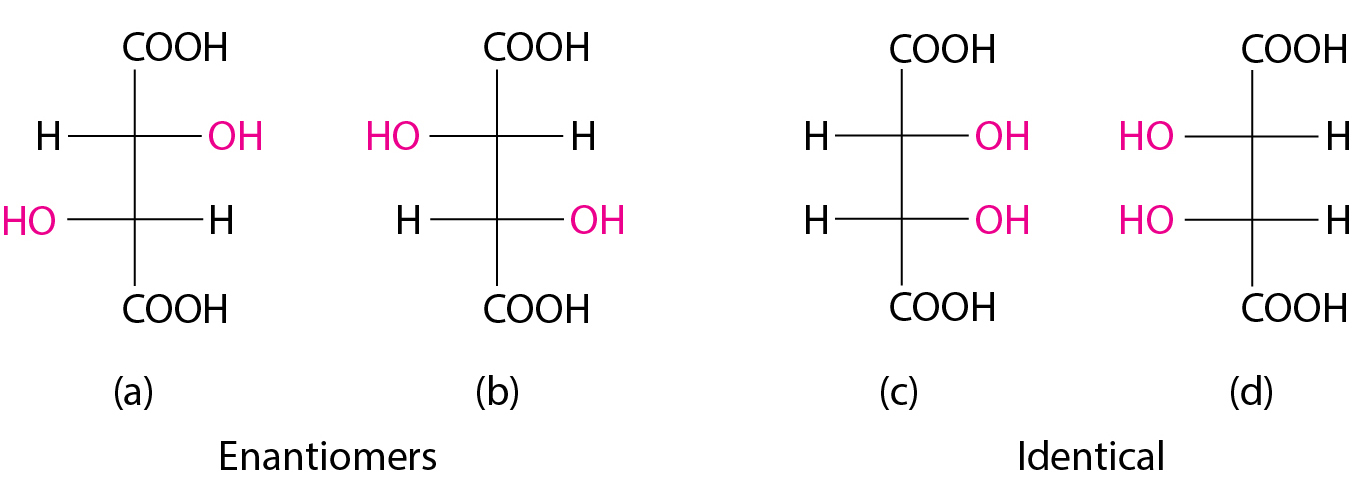
\includegraphics[width=0.7\linewidth]{mesoverbinding}
	\caption[Mesoverbinding]{Enantiomeer (links) en mesoverbinding (rechts)}
	\label{fig:mesoverbinding}
\end{figure}

\begin{figure}[htbp]
	\centering
	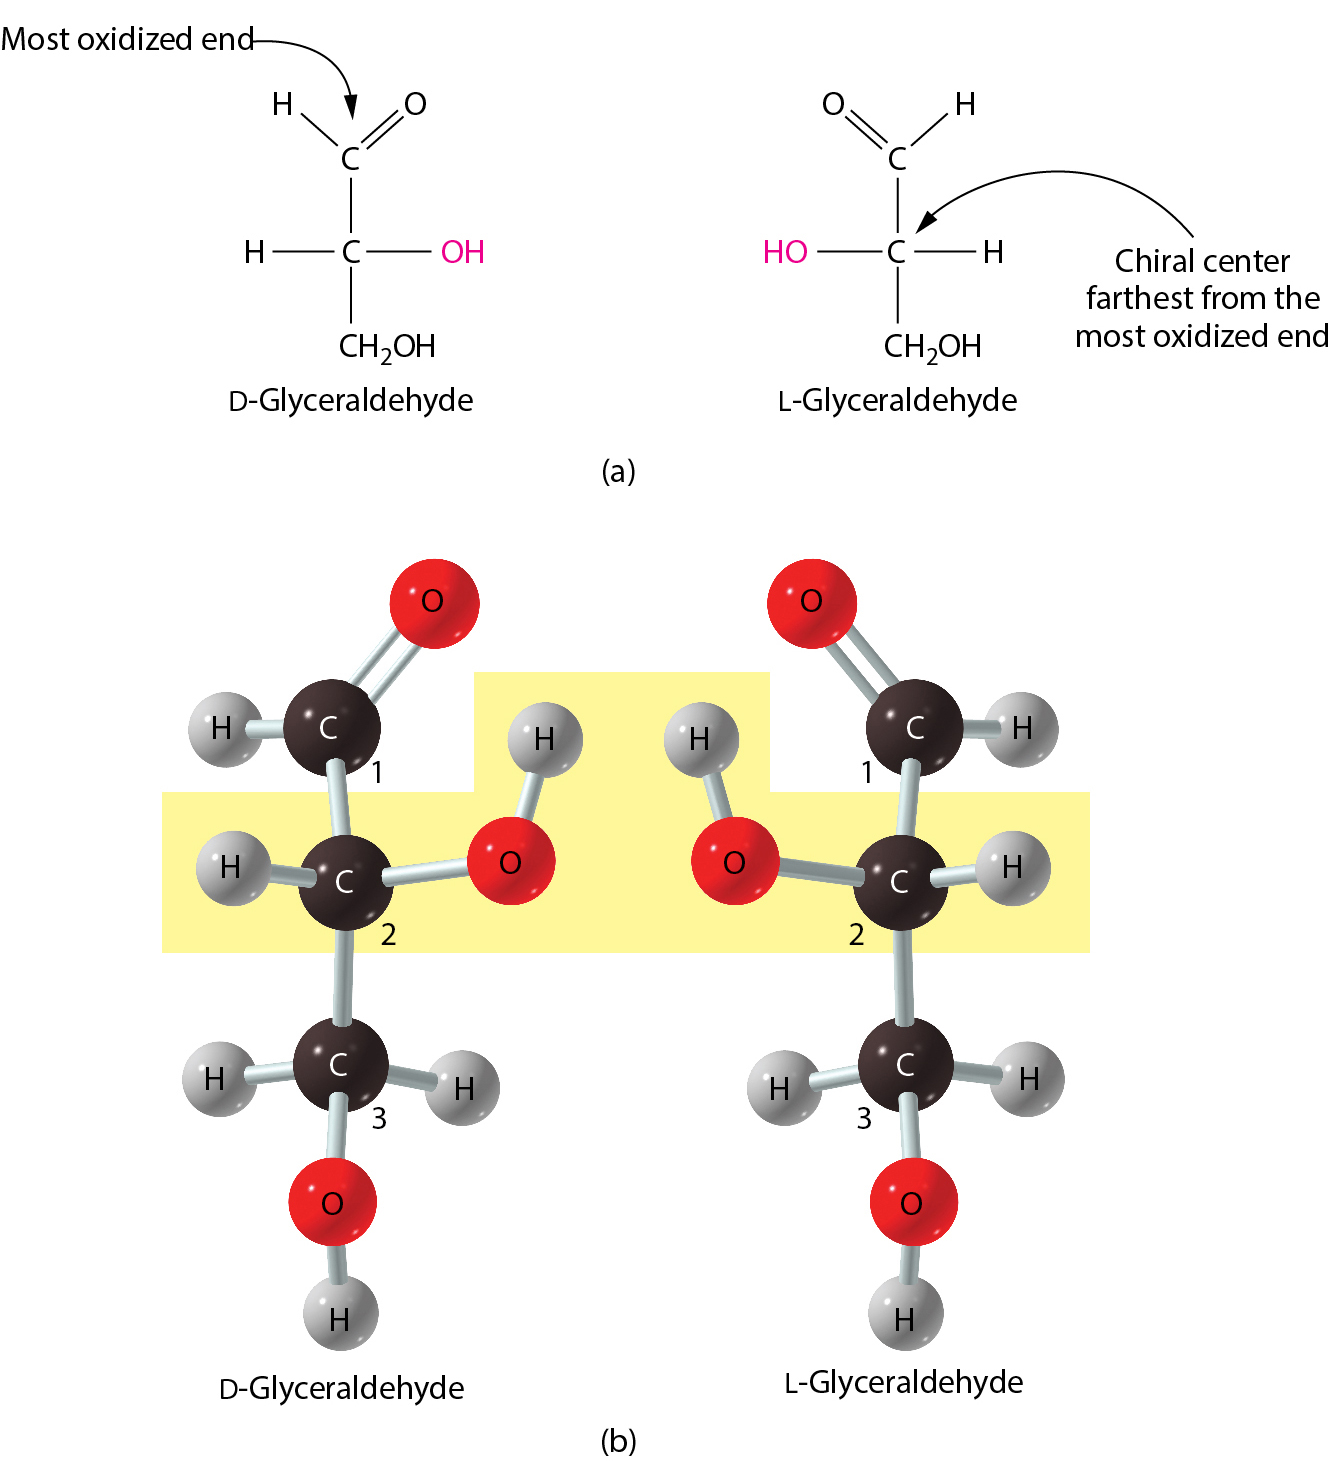
\includegraphics[width=0.6\linewidth]{enantiomeren}
	\caption[Enantiomeer]{Enantiomeer}
	\label{fig:enantiomeren}
\end{figure}
\begin{figure}[htbp]
	\centering
	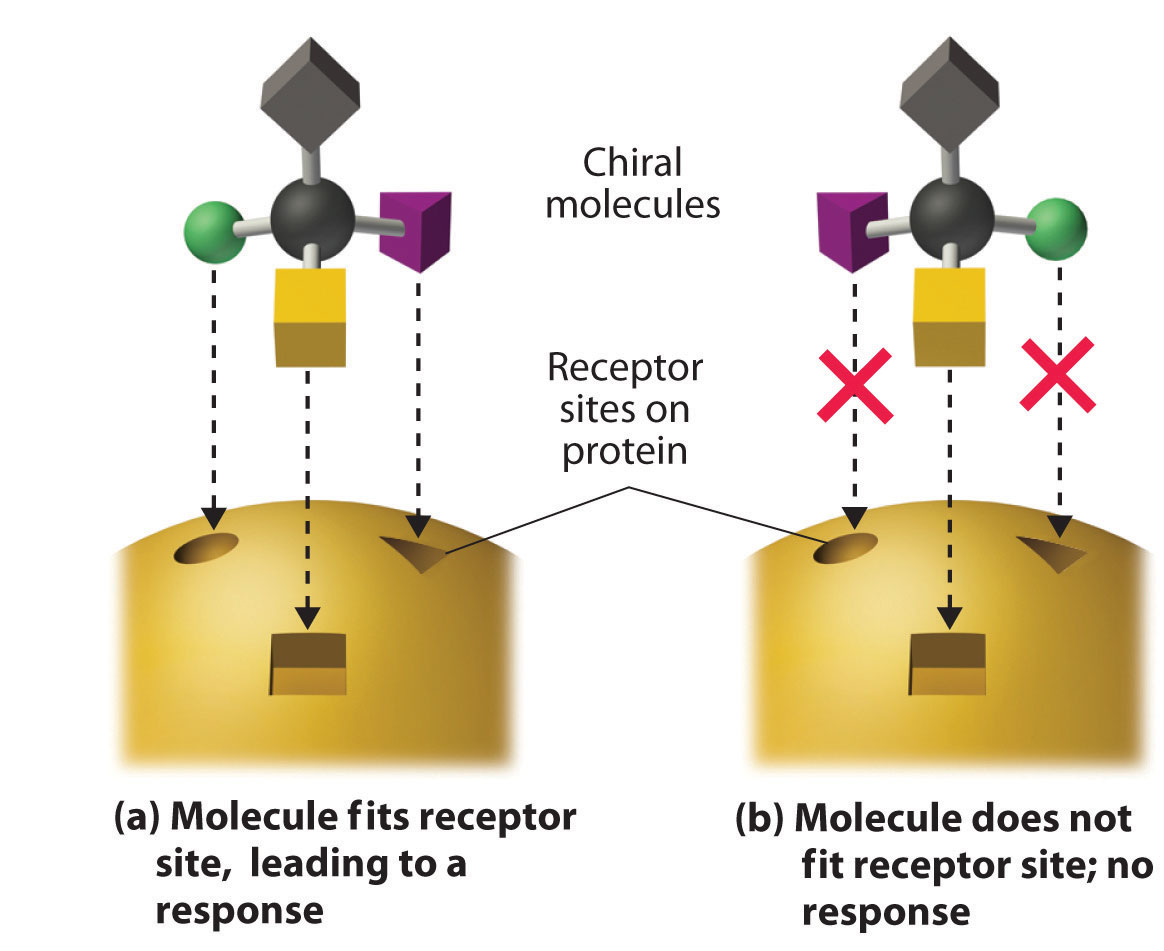
\includegraphics[width=0.5\linewidth]{EnantiomeerEnzym}
	\caption[Enantiomeer en enzym]{Interactie tussen enantiomeren en enzymen}
	\label{fig:enantiomeerenzym}
\end{figure}


\subsubsection{Diastereomeren}
\begin{figure}[htbp]
	\centering
	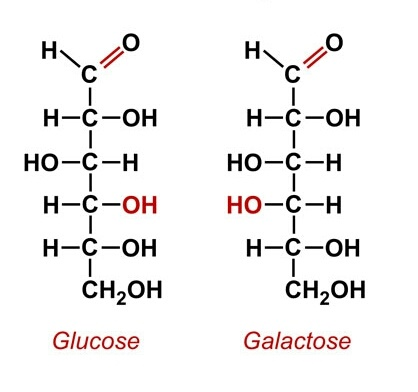
\includegraphics[width=0.4\linewidth]{Diastereomeren}
	\caption[Diastereomeren]{Diastereomeren}
	\label{fig:diastereomeren}
\end{figure}
Diastereomeren zijn zoals enantiomeren, maar ze zijn geen perfect spiegelbeeld zoals te zien is op figuur \ref{fig:diastereomeren}.
\subsubsection{Glucose}
Het bekendste voorbeeld van deze fenomenen is glucose. In de natuur observeren we D-glucose en L-glucose. Hiervan zien we hoofdzakelijk D-glucose voorkomen omdat dit het type glucose is dat gemaakt wordt door fotosynthese. Ons lichaam maakt wel een onderscheid tussen beide varianten, ze smaken alle twee zoet maar enkel D-glucose heeft een calorische inhoud bij het verteren. Dit wil zeggen dat L-glucose niet wordt opgenomen door ons spijsverterings-stelsel, en dus niet kan  gebruikt worden om energie uit te halen. Het is dus een `zoetstof'.

\subsection{Reducerende koolhydraten}
We spreken van een reducerend koolhydraat als het molecuul optreedt als reducerend agens in een reactie als gevolg van de aanwezigheid van de aldehyde- of ketongroep (zie figuur \ref{fig:reductiefding}). Veel monosachariden bezitten deze eigenschap, daarnaast hebben ook disachariden, waarvan het anomere koolstof-atoom geen glycoside binding heeft, ook een reducerend vermogen. Polysachariden hebben meestal een te lage hoeveelheid reducerende uiteinden om een reductief karakter te hebben.
\begin{figure}[htbp]
	\centering
	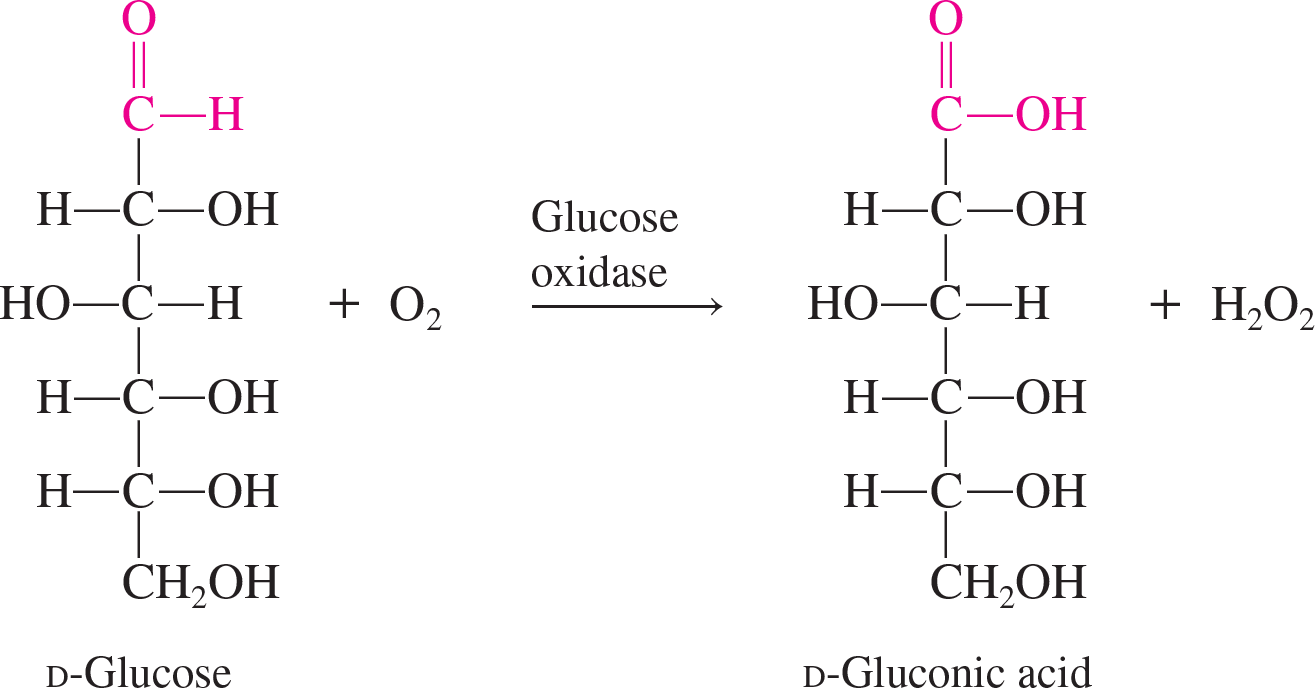
\includegraphics[width=0.5\linewidth]{ReductiefDing}
	\caption[Reducerende koolhydraten]{Reducerende koolhydraten}
	\label{fig:reductiefding}
\end{figure}\\
We kunnen testen of een koolhydraat in het bezit is van een reducerend karakter met Benetict's reagens. Hierbij kijken we naar de kleurverandering van de oplossing na de reactie. Dit is tevens de manier waarop we kunnen bepalen of er suiker in urine zit, het is handig om suikerziekte op te sporen.

\subsection{Monosachariden}
Monosachariden zijn de meest eenvoudige koolhydraten. Ze vormen hierdoor dus ook de bouwstenen voor complexere structuren zoals disachariden en polysachariden. 
\subsubsection{Belangrijke monosachariden}
\textbf{Glucose}
\begin{figure}[h]
	\centering
	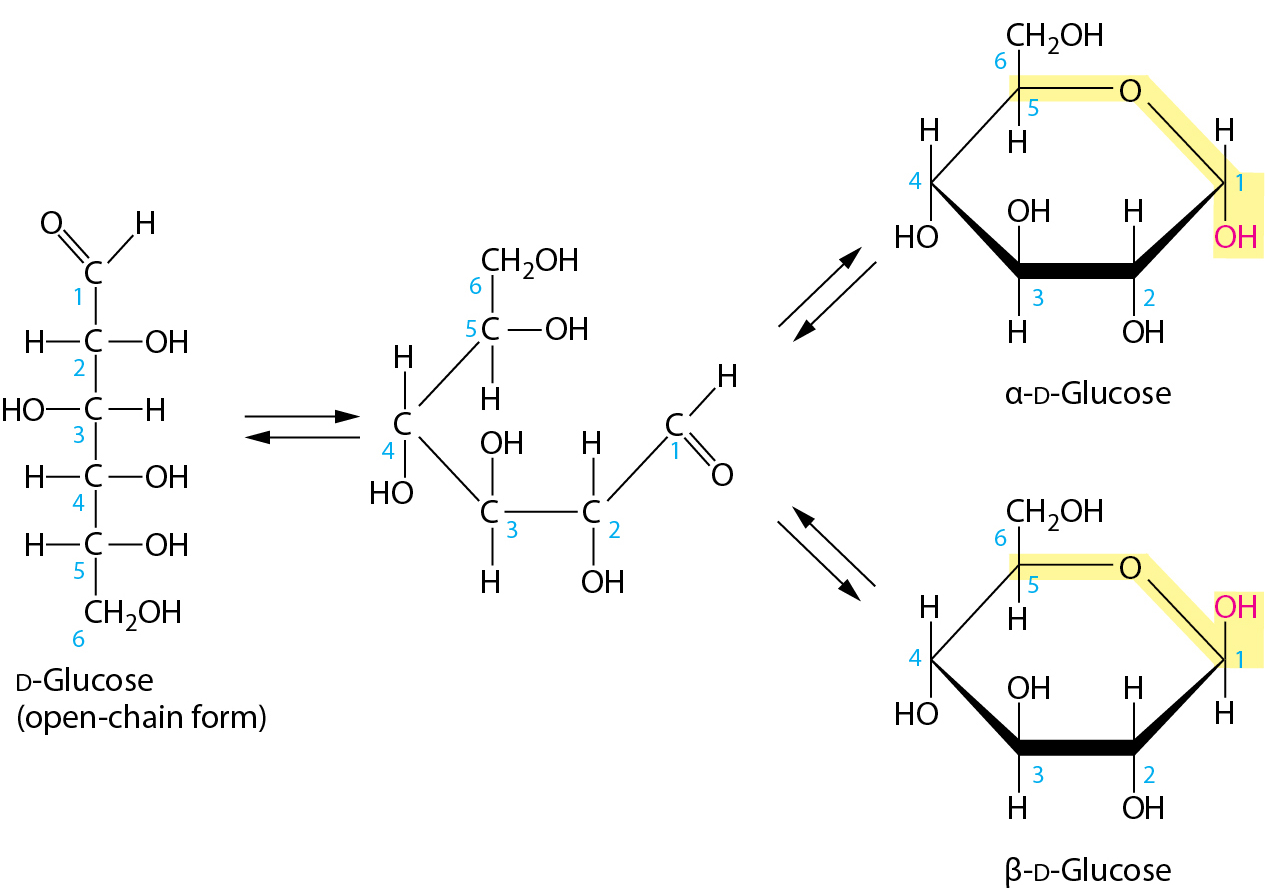
\includegraphics[width=0.7\linewidth]{GlucoseAlphaBeta}
	\caption[Glucose]{Glucose}
	\label{fig:glucosealphabeta}
\end{figure}\\
Hierbij kunnen we nog vermelden dat koolstof atoom 1 in figuur \ref{fig:glucosealphabeta} een nieuw chiraal centrum is, en dus een anomeer C-atoom is.\\
\textbf{Fructose}
\begin{figure}[h]
	\centering
	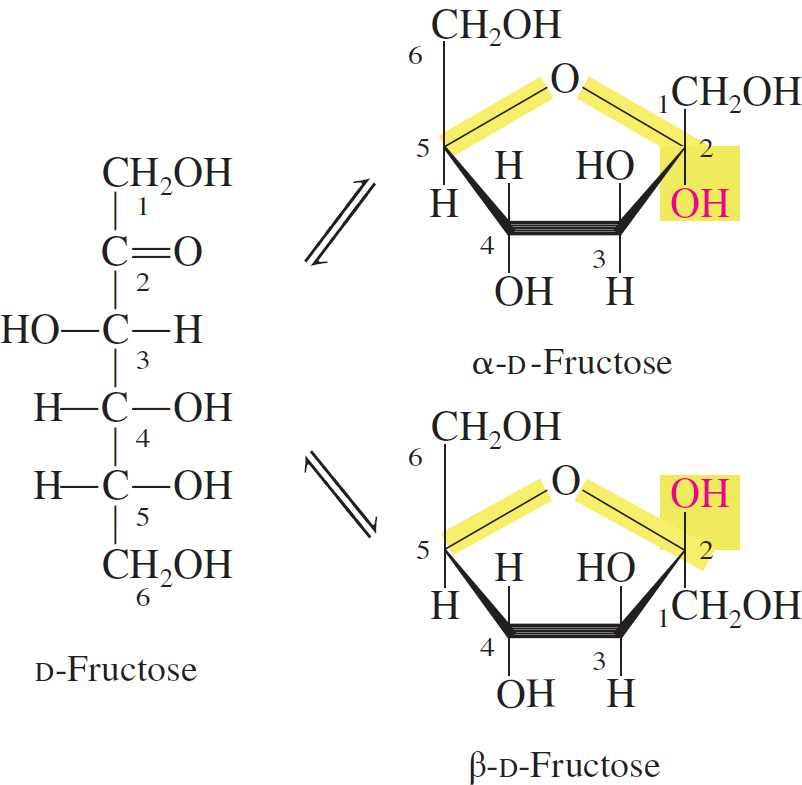
\includegraphics[width=0.4\linewidth]{FructoseAlphaBeta}
	\caption[Fructose]{Fructose}
	\label{fig:fructosealphabeta}
\end{figure}\\
Hierbij kunnen we nog vermelden dat koolstof atoom 2 in figuur \ref{fig:fructosealphabeta} een nieuw chiraal centrum is, en dus een anomeer C-atoom is.\\
\newpage
\textbf{Deoxyribose}
\begin{figure}[h]
	\centering
	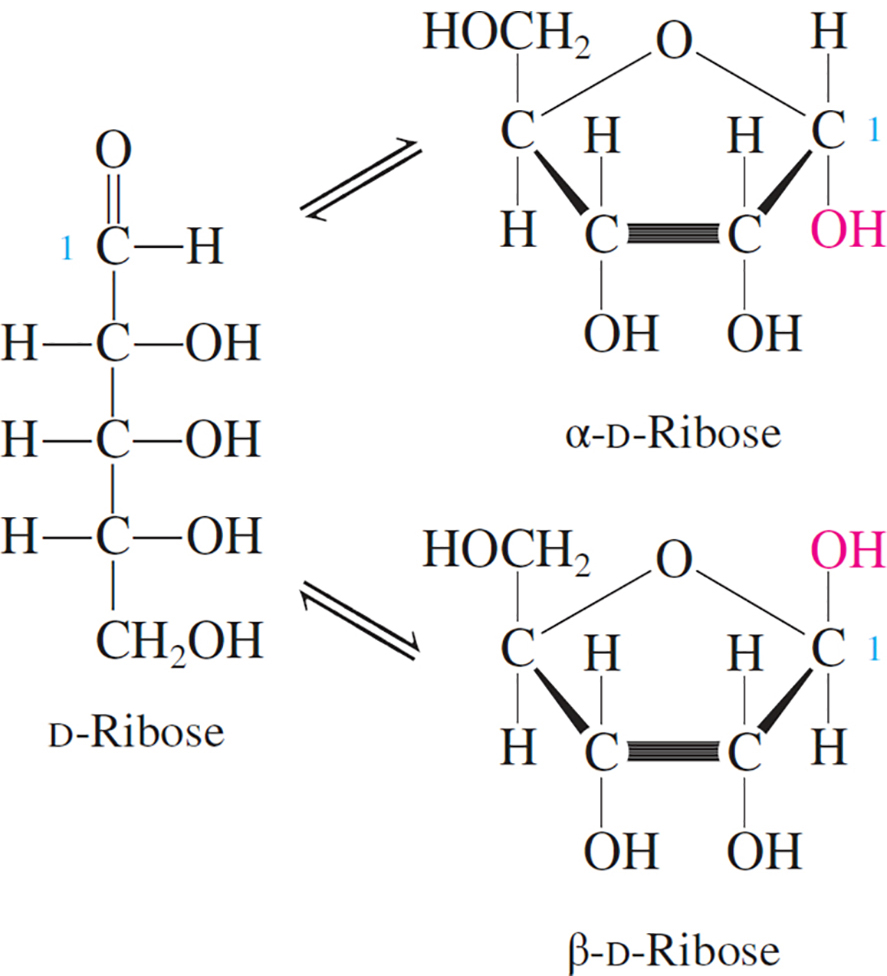
\includegraphics[width=0.4\linewidth]{deoxyribosealphabeta}
	\caption[Deoxyribose]{Deoxyribose}
	\label{fig:deoxyribosealphabeta}
\end{figure}\\
Hierbij kunnen we nog vermelden dat koolstof atoom 1 in figuur \ref{fig:deoxyribosealphabeta} een nieuw chiraal centrum is, en dus een anomeer C-atoom is. Deoxyribose is tevens belangrijk voor RNA en DNA.\\
\textbf{Acetylglucosamine}\\
Door andere functionele groepen toe te voegen aan de koolhydraatstructuur kunnen we complexere moleculen maken. Acetylglucosamine (figuur \ref{fig:acetylglucosamine}) is bijvoorbeeld een bloed antigen.
\begin{figure}[h]
	\centering
	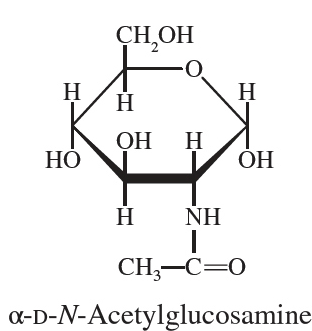
\includegraphics[width=0.4\linewidth]{Acetylglucosamine}
	\caption[Acetylglucosamine]{Acetylglucosamine}
	\label{fig:acetylglucosamine}
\end{figure}
\subsubsection{Afgeleiden}
Enkele voorbeelden van afgeleiden van monosachariden zijn polyolen. Ze zijn geen monosachariden, maar lijken er wel sterk op. De voorbeelden uit figuur \ref{fig:afgeleidenmonosachariden} zijn zoet zoals glucose, ze hebben wel geen calorie-inhoud. Ze zijn dus geschikt om zoetstoffen mee te maken.
\begin{figure}[h]
	\centering
	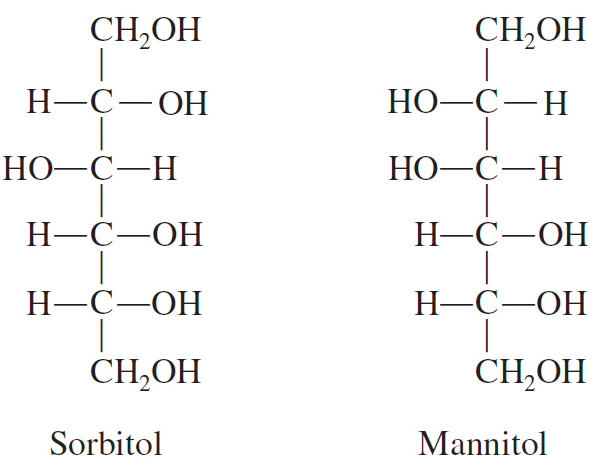
\includegraphics[width=0.4\linewidth]{AfgeleidenMonosachariden}
	\caption[Afgeleiden]{Afgeleiden van monosachariden}
	\label{fig:afgeleidenmonosachariden}
\end{figure}

\subsection{Disachariden}
\subsubsection{Belangrijke disachariden}
\subsection{Polysachariden}
\subsubsection{Belangrijke polysachariden}
\section{Lipiden}
%Overzicht Schema slide 28
\subsection{Biologische functies van lipiden}
\subsection{Vetzuren}
\subsubsection{Structuur}
\subsubsection{(On)Verzadigde vetzuren}
\subsubsection{Cis- en Transvetzuren}
\subsubsection{Omega vetzuren}
\subsubsection{Reacties met vetzuren}
%Mooie samenvatting op slide 16
\subsection{Glyceriden}
\subsubsection{Structuur}
\subsubsection{Triglyceriden}
\subsubsection{Reacties}
\subsubsection{Fosfoglyceriden}
\subsection{Niet-glyceride lipiden}
\subsubsection{Sfingolipide}
\subsubsection{Steroïden}




\end{document}
